% !TeX root = ./LetsDriveDipl.tex
\def \currentAuthor {Nicolas Frey} %so kann jederzeit der Autor geändert werden -> wird in der Fusszeile angezeigt.

\chapter*{Einleitende Bemerkungen}



\chapter*{Notationen}
Beschreibung wie Code, Hinweise, Zitate etc. formatiert werden  



\chapter{Einleitung}



\chapter{Projektmanagement}



\section{Metainformationen}



\subsection{Team}



\subsection{Betreuer}



\subsection{Partner}



\subsection{Ansprechpartner}



\section{Vorerhebungen}
In den Vorerhebungen werden der IST - Zustand und der SOLL - Zustand genau erklärt. Eine Zielformulierung beschreibt das erwartete Ergebnis eindeutig, attraktiv, realistisch und messbar mit konkreten Terminen. Einfluss, Nähe und Einstellung der Stakeholder und Maßnahmen für diese werden graphisch und tabellarisch dargestellt.



\subsection{Projektzieleplan}
Ziel ist die Erstellung einer Smartphone-App für Fahrschüler:innen, welche über GPS - Tracking automatisch Einträge in einem Fahrtenbuch aufzeichnet. Diese Einträge sollen in Form eines offiziellen Protokolls an die Fahrschule ausgehändigt werden können. Um Schüler:innen besser auf die praktische Fahrprüfung vorzubereiten, soll ebenso ein digitaler Fahrlehrer implementiert werden, dem/der Schüler:in Feedback in Form von statistischen Auswertungen gibt. Bis zum 28.6.2024 sollen alle oben genannten Features implementiert, getestet und veröffentlicht werden. Um sich ein Bild vom Markterfolg machen zu können, werden hierbei die App-Store Bewertungen und Downloadzahlen verwendet. Das Ziel ist, bis September die 3\%-Schwelle zu erreichen, das bedeutet etwa 100 Neukunden unter allen Österreicher:innen, die die L-Tafel beantragen (einschließlich L-17).



\subsubsection*{IST-Zustand}
Bis dato gibt es keine App, die das Aufzeichnen des Fahrtenbuchs für den Führerschein mit L-Tafel unabhängig von Fahrschulen und Mitgliedschaften (ÖAMTC) ermöglicht. Des Weiteren gibt es kein weitverbreitetes Tool das dem/der Fahrschüler:in personalisiertes Feedback seines/r bisherigen 



\subsubsection*{SOLL-Zustand}
Eine Smartphone-App für Fahrschüler:innen, welche über GPS - Tracking automatisch Einträge in einem Fahrtenbuch erstellt. Diese Einträge werden in Form eines offiziellen Protokolls exportiert. Das Analysieren der Fahrdaten und Erzeugen von Statistiken geben dem/der Fahrschüler:in ein Feedback. Zur Datensicherung steht eine Datenbank zur Verfügung.

\subsection{Projektumfeld}

\subsubsection*{Identifikation der Stakeholder}
Zu Beginn haben wir mittels „Brainstorming“ die wichtigsten Stakeholder identifiziert. Uns wurde ersichtlich, dass nur User also Fahrschüler:innen und Begleitpersonen unsere Zielgruppen sind und mit dem Produkt zufrieden sein müssen. Im Laufe der Recherche wurde eine von ÖAMTC bereitgestellte\hfill\break Konkurrenz-App identifiziert, wodurch uns sofort klar war, dass wir gleich von Beginn an ein starkes Auftreten brauchen. Das bedeutet, dass wir speziell durch bessere Software und Features, sowie durch ein besseres Preismodell attraktiver für den Kunden sein wollen. Die Stakeholder werden mithilfe der folgenden Tabellen und Abbildungen (\cref{tab:Charakterisierung}, \cref{tab:Maßnahmen}, \cref{fig:Stakeholder}) dargestellt.



\subsubsection*{Charakterisierung der Stakeholder}
\begin{table}[H]
	\centering
	\begin{tabular}{|c|c|c|c|p{4.4cm}|}
		\hline
		\textbf{Stakeholder} & \textbf{Einfluss} & \textbf{Nähe} & \textbf{Einstellung} & \textbf{Beschreibung} \\
		\hline
		Auftraggeber & groß & nahe & positiv & Geschäftsführer \\
		\hline
		Fahrschulen & groß & mittel & neutral & Die Fahrschulen, welche die Fahrschüler:innen ausbilden. \\
		\hline
		Begleitperson & groß & nahe & positiv & z.B Eltern der Fahrschüler:innen \\
		\hline
		Fahrschüler:innen & groß & nahe & positiv & Die Fahrschüler:innen selbst \\
		\hline
		Medien & gering & mittel & neutral & Alle Medien die Über diese App berichten. \\
		\hline
		Konkurrenz-Apps & groß & nahe & negativ & Konkurrenz-Apps z. Bsp.: ÖAMTC \\
		\hline
	\end{tabular}
	\caption{Charakterisierung der Stakeholder}
	\label{tab:Charakterisierung}

\end{table}



\subsubsection*{Maßnahmen}
\begin{table}[H]
	\centering
	\begin{tabular}{|c|p{10.6cm}|}
		\hline
		\textbf{Stakeholder} & \textbf{Maßnahmen} \\
		\hline
		Auftraggeber & Wöchentliche Meetings. Berichte und Fortschritte liefern. \\
		\hline
		Fahrschulen & Überzeugen, dass das Protokoll weniger leicht verfälscht werden kann und die App die Fahrschüler:innen unterstützt. \\
		\hline
		Begleitperson & Protokollierung mittels App soll eine Erleichterung sein und Schutz vor Datenverlust bieten. \\
		\hline
		Fahrschüler:innen & Positive Werbung, benutzerfreundliches und praktisches Design der App, sowie werbungsfrei. \\
		\hline
		Medien & Durch Erfolg und hohe Userzahlen, sowie gutes Marketing / auf App aufmerksam machen. \\
		\hline
		Konkurrenz-Apps & Faires Konkurrenzverhalten \\
		\hline
	\end{tabular}
	\caption{Maßnahmenkatalog}
	\label{tab:Maßnahmen}
\end{table}



\subsubsection*{Grafische Darstellung des Umfeldes}
\begin{figure}[H]
	\centering
	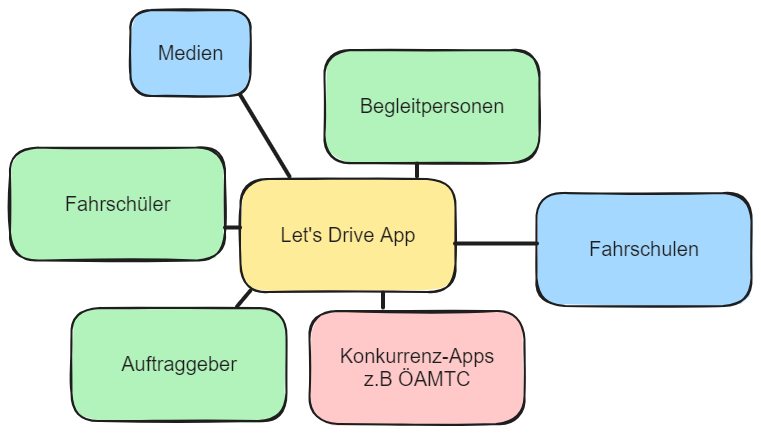
\includegraphics[width=15cm]{figures/graf_stakeholder.png}
	\caption{Grafik Stakeholder}
	\label{fig:Stakeholder}
\end{figure}


\subsection{Risikoanalyse}

\begin{itemize}
	\item Risikomatrix
\end{itemize}



\section{Problemanalyse}



\subsection{USE-Case-Analyse}
\begin{itemize}
	\item UseCases auf Basis von Benutzerzielen identifizieren:
	      \begin{itemize}
		      \item Benutzer eines Systems identifizieren
		      \item Benutzerziele identifizieren (Interviews)
		      \item Use-Case-Liste pro Benutzer definieren
	      \end{itemize}
	\item UseCases auf Basis von Ereignissen identifizieren:
	      \begin{itemize}
		      \item Externes Event triggert einen Prozess
		      \item zeitliches Event triggert einen Prozess (Zeitpunkt wird erreicht)
		      \item State-Event (Zustandsänderung im System triggert einen Prozess)
	      \end{itemize}
	\item Werkzeuge:
	      \begin{itemize}
		      \item USE-Case-Beschreibungen (textuell, tabellarisch)
		      \item USE-Case-Diagramm
		      \item Aktivitätsdiagramm für den Use-Case (Interaktion zwischen Akteur und System abbilden)
		      \item System-Sequenzdiagramm (Spezialfall eines Sequenzdiagramms: Nur 1 Akteur und 1 Objekt, das Objekt ist das komplette System, es geht um die Input/Output Requirements, die abzubilden sind)
	      \end{itemize}
\end{itemize}

\subsection{Domain-Class-Modelling}



\begin{itemize}
	\item "Dinge" (Rollen, Einheiten, Geräte, Events etc.) identifizieren, um die es im Projekt geht
	\item ER-Modellierung oder Klassendiagramme
	\item Zustandsdiagramme (zur Darstellung des Lebenszyklus von Domain-Klassen darstellen)
\end{itemize}

\subsection{User-Interface-Design}
\begin{itemize}
	\item Mockups
	\item Wireframes
\end{itemize}

\section{Pflichtenheft}

\subsection{Zielbestimmung}
\begin{itemize}
	\item Projektbeschreibung
	\item IST-Zustand
	\item SOLL-Zustand
	\item NICHT-Ziele (Abgrenzungskriterien)
\end{itemize}
\subsection{Produkteinsatz und Umgebung}
\begin{itemize}
	\item Anwendungsgebiet
	\item Zielgruppen
	\item Betriebsbedingungen
	\item Hard-/Softwareumgebung
\end{itemize}
\subsection{Funktionalitäten}
\begin{itemize}
	\item MUSS-Anforderungen
	      \begin{itemize}
		      \item Funktional
		      \item Nicht-funktional
	      \end{itemize}
	\item KANN-Anforderungen
	      \begin{itemize}
		      \item Funktional
		      \item Nicht-funktional
	      \end{itemize}
\end{itemize}
\subsection{Testszenarien und Testfälle}
\begin{itemize}
	\item Beschreibung der Testmethodik
	\item Testfall 1
	\item Testfall 2
	\item \ldots
\end{itemize}
\subsection{Liefervereinbarung}
\begin{itemize}
	\item Lieferumfang
	\item Modus
	\item Verteilung(Deployment)
\end{itemize}
\section{Planung}
\subsection{Projektstrukturplan}
\subsection{Meilensteine}
\subsection{Ablaufplanung}
Gantt-Chart
\subsection{Abnahmekriterien}
\subsection{Pläne zur Evaluierung}
\subsection{Ergänzungen und zu klärende Punkte}

\chapter{Vorstellung des Produktes}
Vorstellung des fertigen Produktes anhand von Screenshots, Bildern, Erklärungen.

\chapter{Eingesetzte Technologien}
\begin{itemize}
	\item Kurzbeschreibung aller Technologien, die verwendet wurden.
	\item Technologien die aus dem Unterricht bekannt sind, nur nennen und deren  Einsatzzweck im Projekt beschreiben, nicht die Technologien selbst.
	\item Technologien die aus dem Unterricht nicht bekannt sind, im Detail beschreiben incl. deren Einsatz im Projekt
	\item Fokus aus eingesetzten Frameworks
\end{itemize}

\chapter{Systementwurf}

\section{Architektur}

\subsection{C4 - Modell}

Beschreibung der Architektur der Software unter Verwendung des C4 Modells: \url{https://c4model.com/}.

Darstellung und Beschreibung der Systemarchitektur.

\begin{itemize}
	\item  statische Zerlegung des Systems in seine physischen Bestandteile (Komponenten, Komponentendiagramm)
	\item (textuelle) Beschreibung des dynamischen Zusammenwirkens aller Komponenten
	\item (textuelle) Beschreibung der Strategie für die Architektur, d. h. wie die Architektur in Statik und Dynamik funktionieren soll.
	\item Verwendung von Referenzarchitekturen bzw. Architekturmustern (als Schablonen, z.B. MVC. Plugin, Pipes and Filters)
	      \begin{itemize}
		      \item MVC
		      \item Schichten
		      \item Pipes
		      \item Request Broker
		      \item Service-Oriented
	      \end{itemize}
\end{itemize}

\subsection{Benutzerschnittstellen}
\begin{itemize}
	\item Design des UIs
	\item Dialoge, Dialogsteuerung, Ergonomie, Gestaltung, Eingabeüberprüfungen
\end{itemize}

\subsection{Datenhaltunskonzept}
\begin{itemize}
	\item Design der Datenbank (ER-Modell)
	\item Design des Zugriffs auf diese Daten (Datenhaltungskonzept)
	\item Caching, Transaktionen
\end{itemize}

\subsection{Konzept für Ausnahmebehandlung}
\begin{itemize}
	\item Systemweite Festlegung, wie mit Exceptions umgegangen wird
	\item Exceptions sind primär aus den Bereichen UI, Persistenz, Workflow-Management
\end{itemize}

\subsection{Sicherheitskonzept}
Beschreibung aller sicherheitsrelevanten Designentscheidungen

\begin{itemize}
	\item Design der Security-Elemente
	\item Design von Safety-Elementen (Fehlertoleranz, Verfügbarkeit etc.)
\end{itemize}

\subsection{Design der Testumgebung}
\begin{itemize}
	\item wie wird getestet (Unit-Testing, Integrationstesting, Systemtests, Akzeptanztests)
	\item Testumgebung, Testprozess, Teststrategie, Testmethoden, Testfälle
\end{itemize}


\subsection{Desing der Ausführungsumgebung}
\begin{itemize}
	\item Deployment (DevOps)
	\item Betrieb (besonders Hoch- und Hertunerfahren der Anwendung)
\end{itemize}

\section{Detailentwurf}

Design jedes einzelnen USE-Cases

\begin{itemize}
	\item Design-Klassendiagramme vom Domain-Klassendiagramm ableiten (incl. detaillierter Darstellung und Verwendung von Vererbungshierarchichen, abstrakten Klassen, Interfaces)
	\item Sequenzdiagramme vom System-Sequenz-Diagramm ableiten
	\item Aktivitätsdiagramme
	\item Detaillierte Zustandsdiagramme für wichtige Klassen
\end{itemize}

Verwendung von CRC-Cards (Class, Responsibilities, Collaboration) für die Klassen
\begin{itemize}
	\item um Verantwortlichkeiten und Zusammenarbeit zwischen Klassen zu definieren und
	\item um auf den Entwurf der Geschäftslogik zu fokussieren
\end{itemize}

Design-Klassen für jeden einzelnen USE-Case können z.B. sein:

\begin{itemize}
	\item UI-Klassen
	\item Data-Access-Klassen
	\item Entity-Klassen (Domain-Klassen)
	\item Controller-Klassen
	\item Business-Logik-Klassen
	\item View-Klassen
\end{itemize}

Optimierung des Entwurfs (Modularisierung, Erweiterbarkeit, Lesbarkeit):

\begin{itemize}
	\item Kopplung optimieren
	\item Kohäsion optimieren
	\item SOLID
	\item Entwurfsmuster einsetzen
\end{itemize}

\chapter{Implementierung}
Detaillierte Beschreibung der Implementierung aller Teilkomponenten der Software entlang der zentralsten Use-Cases:

\begin{itemize}
	\item GUI-Implementierung
	\item Controllerlogik
	\item Geschäftslogik
	\item Datenbankzugriffe
\end{itemize}

Detaillierte Beschreibung der Teststrategie (Testdriven Development):

\begin{itemize}
	\item UNIT-Tests (Funktional)
	\item Integrationstests
\end{itemize}

Zu Codesequenzen:
\begin{itemize}
	\item kurze Codesequenzen direkt im Text (mit Zeilnnummern auf die man in der Beschreibung verweisen kann)
	\item lange Codesequenzen in den Anhang (mit Zeilennummer) und darauf verweisen
\end{itemize}

\chapter{Deployment}
\begin{itemize}
	\item Umsetzung der Ausführungsumgebung
	\item Deployment
	\item DevOps-Thema
\end{itemize}

\chapter{Tests}

\section{Systemtests}
Systemtests aller implementierten Funktionalitäten lt. Pflichtenheft
\begin{itemize}
	\item Beschreibung der Teststrategie
	\item Testfall 1
	\item Testfall 2
	\item Tesfall 3
	\item …
\end{itemize}

\section{Akzeptanztests}

\chapter{Projektevaluation}
siehe Projektmanagement-Unterricht

\chapter{Benutzerhandbuch}
falls im Projekt gefordert

\chapter{Betriebswirtschaftlicher Kontext}
BW-Teil

\chapter{Zusammenfassung}
Mit der Projektumfeldanalyse wurden alle Stakeholder erfasst, die bei einer praktisch ausgelegten App für L17 Fahrschüler:innen als relevant erschienen. Die Positionen der einzelnen Interessensgruppen wurden analysiert und grafisch dargestellt. Weiters wurde ein Maßnahmenkatalog erstellt, um mögliche Methoden zu identifizieren, die das Projektumfeld verbessern sollen. Da dieses Projekt mit der Diplomarbeit am IT-Kolleg zusammenhängt ist der Termin mit Ende Juni für ein Minimum Viable Produkt festgelegt. Dieser Termin ist aber sehr realistisch. Die Anforderungen an diese App sind für eine Smartphone App umfangreich und erfordern eine genaue Auswertung und Prüfung in der Testphase. Dieses Produkt bietet dem/der Fahrschüler:in eine Erleichterung bei der Protokollierung und laufend Feedback über den praktischen Fortschritt dem/der Schüler:in.